\documentclass[12pt,xcolor=svgnames]{beamer} 
\usepackage{fancyvrb}
\usepackage{moreverb}
\usepackage{relsize}
\usepackage{hyperref}

%\usecolortheme[named=Brown]{structure} 
%\useoutertheme{infolines}
%\usetheme{Madrid}

\usefonttheme{serif}
\setbeamertemplate{items}[ball] 
\setbeamertemplate{blocks}[rounded][shadow=true] 
\setbeamertemplate{navigation symbols}{}
\setbeamercolor{normal text}{bg=Cornsilk}

\setbeamertemplate{footline}{%
\hfill\usebeamertemplate***{navigation symbols}
\hspace{1cm}\insertframenumber{}/\inserttotalframenumber \hspace*{5mm}}

\logo{
\includegraphics[height=5mm]{images/bbklogo}}
%
\fvset{tabsize=2}
\fvset{fontsize=\relsize{-1}}
\fvset{frame=single}
\begin{document}
\title{Concurrent Programming}
\subtitle{though Actors and Erlang\\
Functional Programming meets Logic Programming}
\author{Keith Mannock, Sven Helmer, Bruce Tate}
\begin{frame}[plain] 
  \titlepage
  \centerline{
\includegraphics[scale=0.9]{images/erlang-logo.png}}
  \end{frame}
  
\begin{frame}[fragile,allowframebreaks]{Overview}
\begin{itemize}
\item Concurrency, parallelism, and mutable shared data
\item Concurrent computation using the Actor Model
\item Elixir, Erland, and the Akka Framework as an Actor Model implementation	
\end{itemize}

\framebreak

\begin{itemize}
\item Threads, concurrency, and parallelism
\item Shared data and mutability
\item Synchronisation to the rescue
\item Why concurrent programming is hard	
\end{itemize}

\end{frame}

\begin{frame}[fragile,allowframebreaks]{Serial vs. Parallel}

\begin{itemize}
\item The programming world used to be much simpler place
\begin{itemize}
\item Almost all programs ran in a serial fashion on a single CPU
\item A programmer would not have to deal with parallelism or concurrency 
\end{itemize}
\item Developers could rely on the fact that more powerful CPUs would appear, making their code run faster
\end{itemize}

\framebreak

\begin{itemize}

\item However, things have changed:
\begin{itemize}
\item At some point we will reach the limits of Moore's law
\item Designers of CPUs are facing severe problems with power dissipation (due to high integration)
\end{itemize}
\item One solution to these problems is to build multi-core and/or distributed systems
\item In order to fully exploit these systems, programmers have to embrace a different programming style
\end{itemize}
\end{frame}


\begin{frame}{Threads, Concurrency, and Parallelism}
\centerline{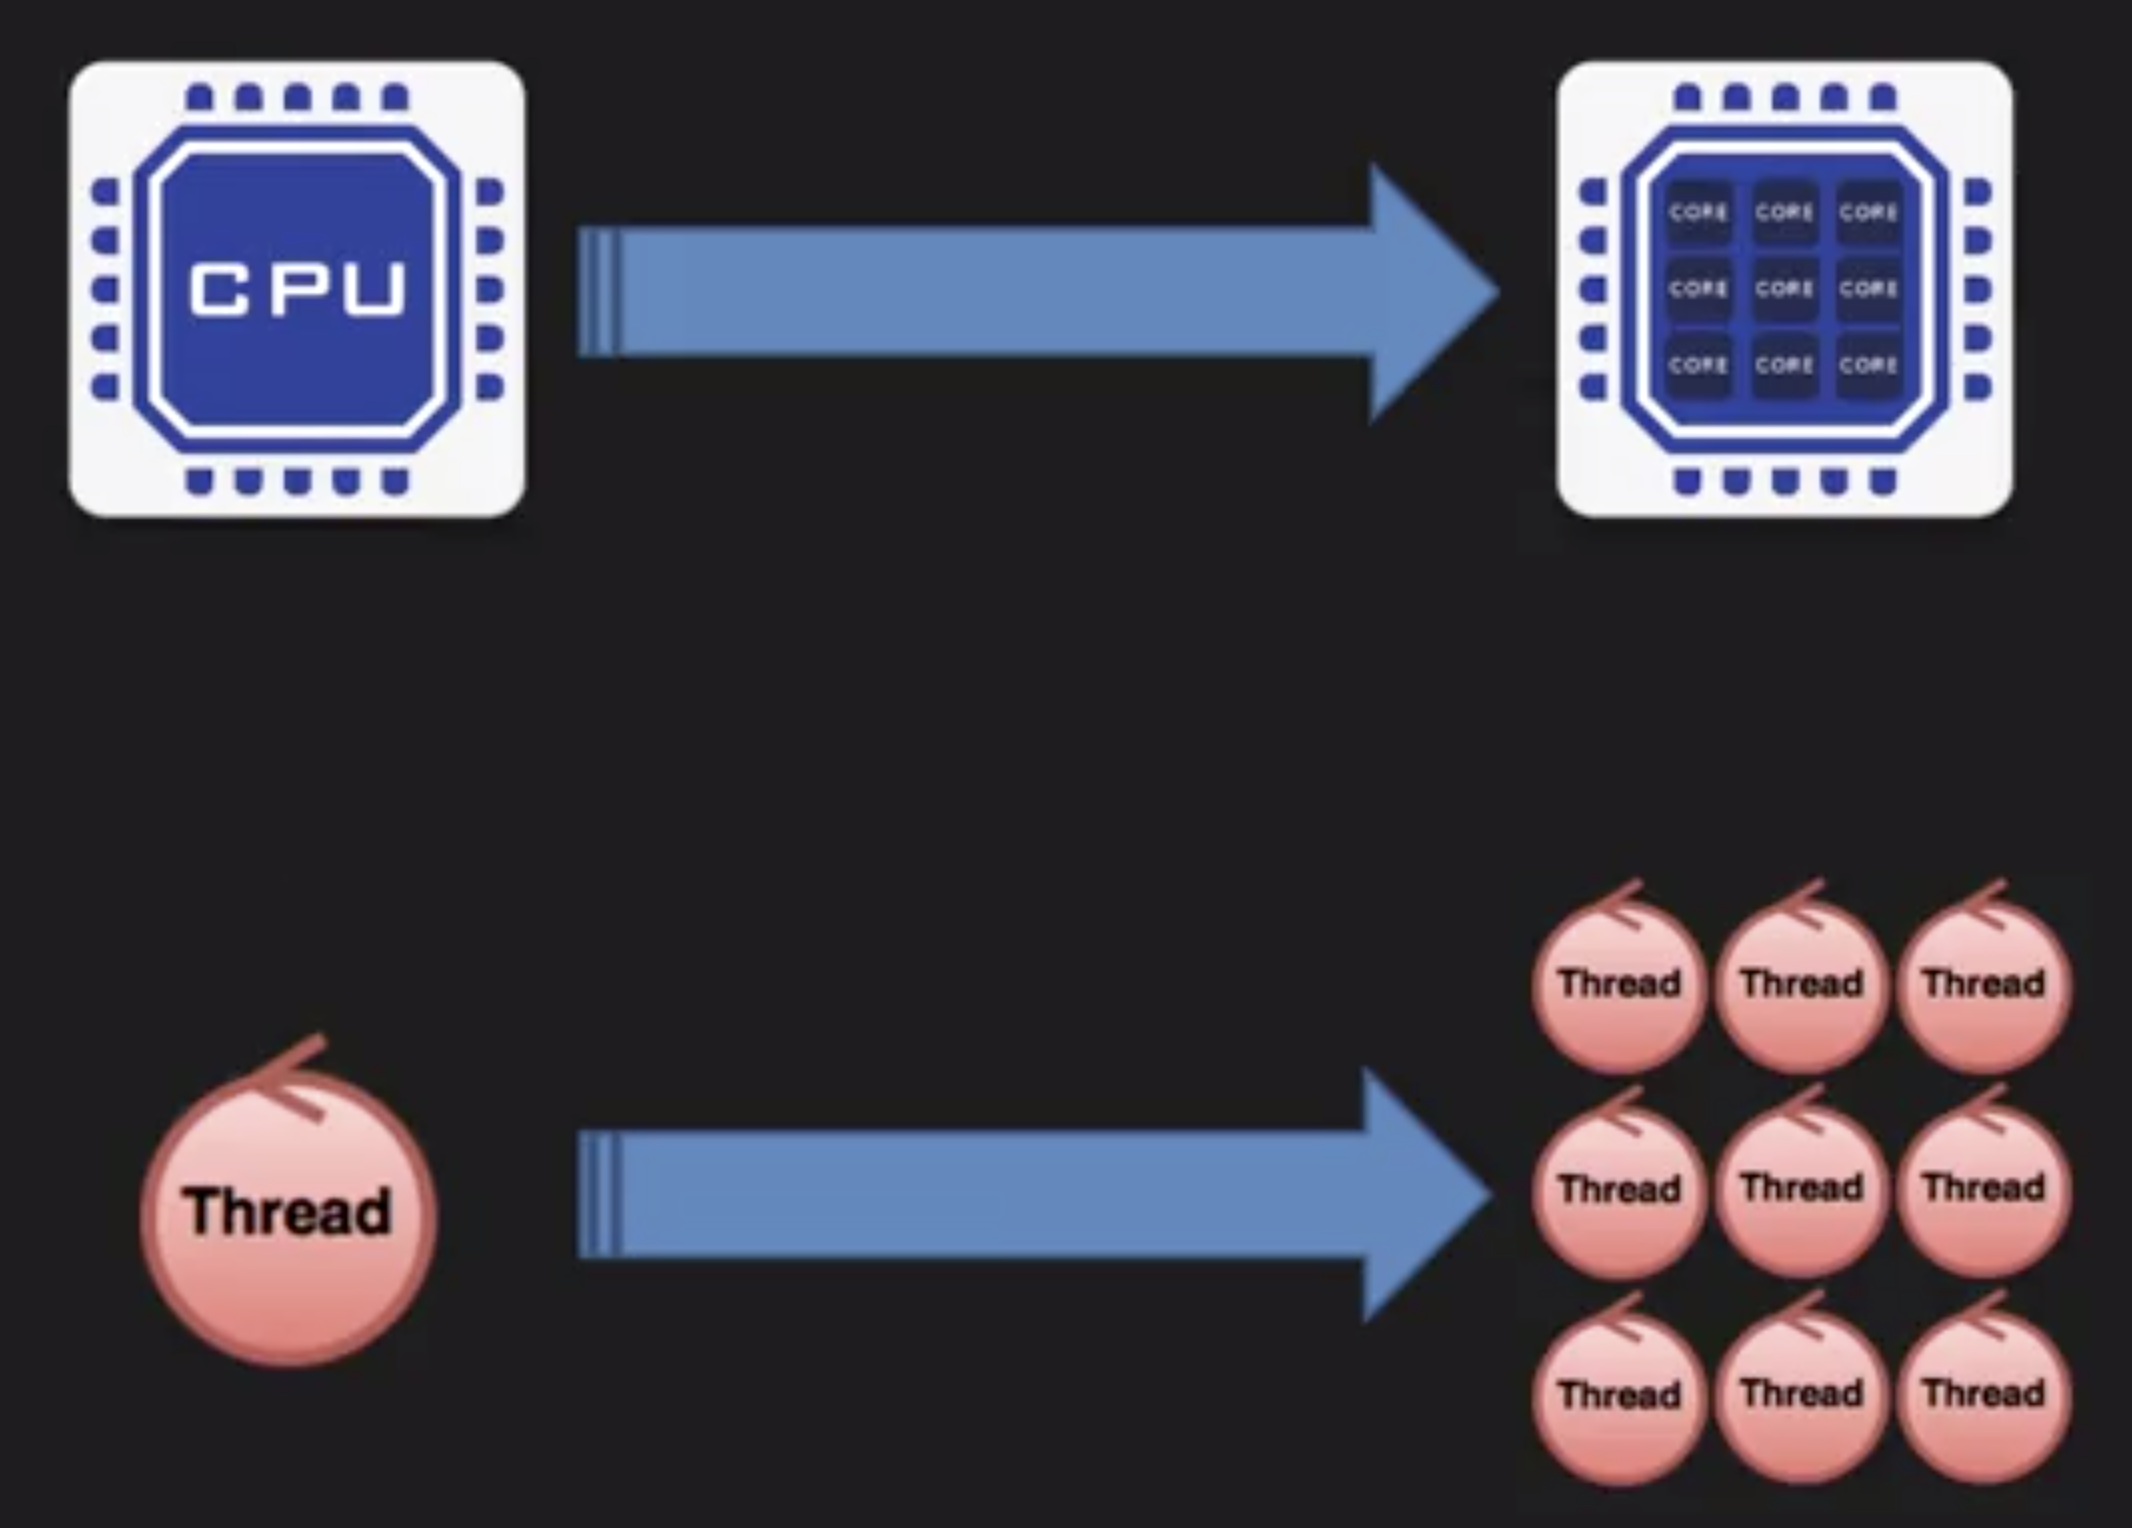
\includegraphics[width=0.75\textwidth]{images/threads}}	
\end{frame}

\begin{frame}[fragile,allowframebreaks]{Multi-threaded Programming}
\begin{itemize}
\item In many programming languages, such as Java or C++, threads were introduced to \alert{parallelise} programs
\item This should lead to better performance, as multiple cores can actually be utilised
\item However, there is a downside to multi-threading
\item Threads share resources:
\begin{itemize}
\item Resource contention leads to bottlenecks
\item Writing (and debugging) multi-threaded code is very complex
\end{itemize}
\end{itemize}

\framebreak

\begin{center}
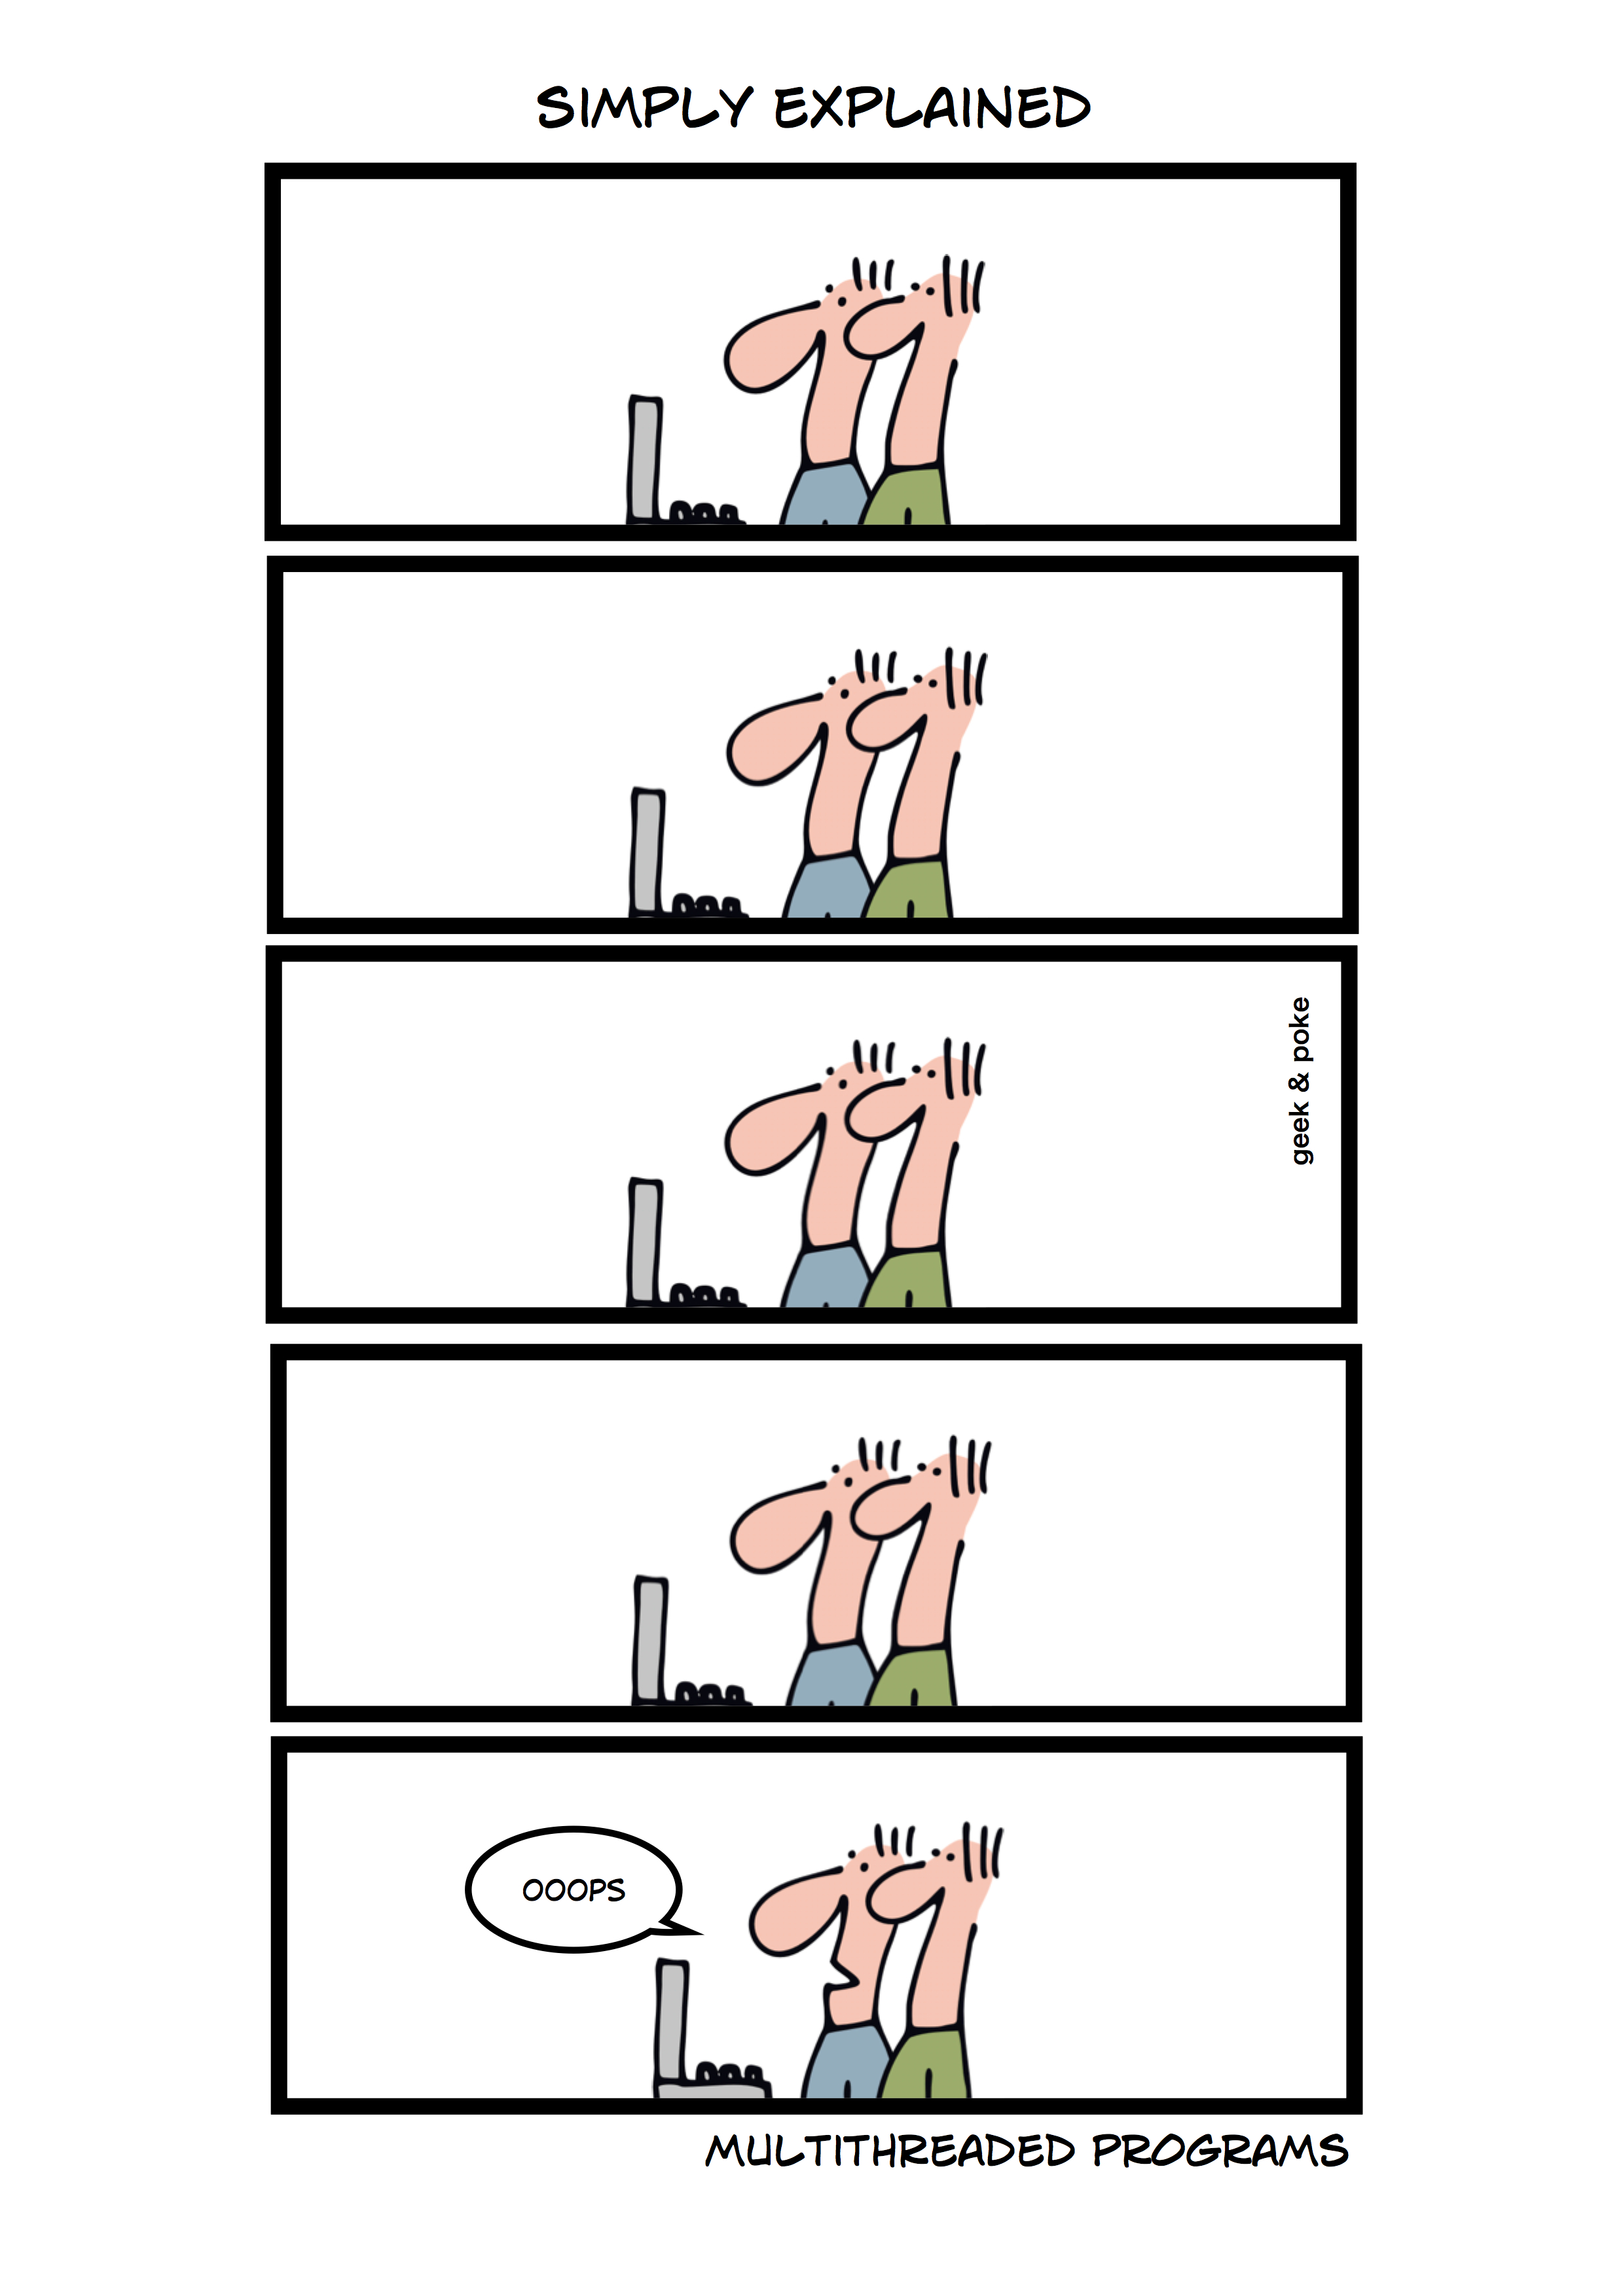
\includegraphics[height=0.85\textheight]{images/multithreaded.png}
\end{center}
\end{frame}

\begin{frame}{Concurrency}
A somewhat informal definition of concurrency

\begin{itemize}
\item Put simply, \emph{concurrent} means that tasks can be done in any order without compromising the results
\begin{itemize}
\item For example, (separately) shuffling two decks of cards: can be done in any order or even in parallel
\end{itemize}
\item This is not the same as parallelism, concurrent tasks do not have to be done in parallel
\item However, we can run them in parallel without any negative effects
\end{itemize}
\end{frame}

\begin{frame}{Shared data and mutability}
\centerline{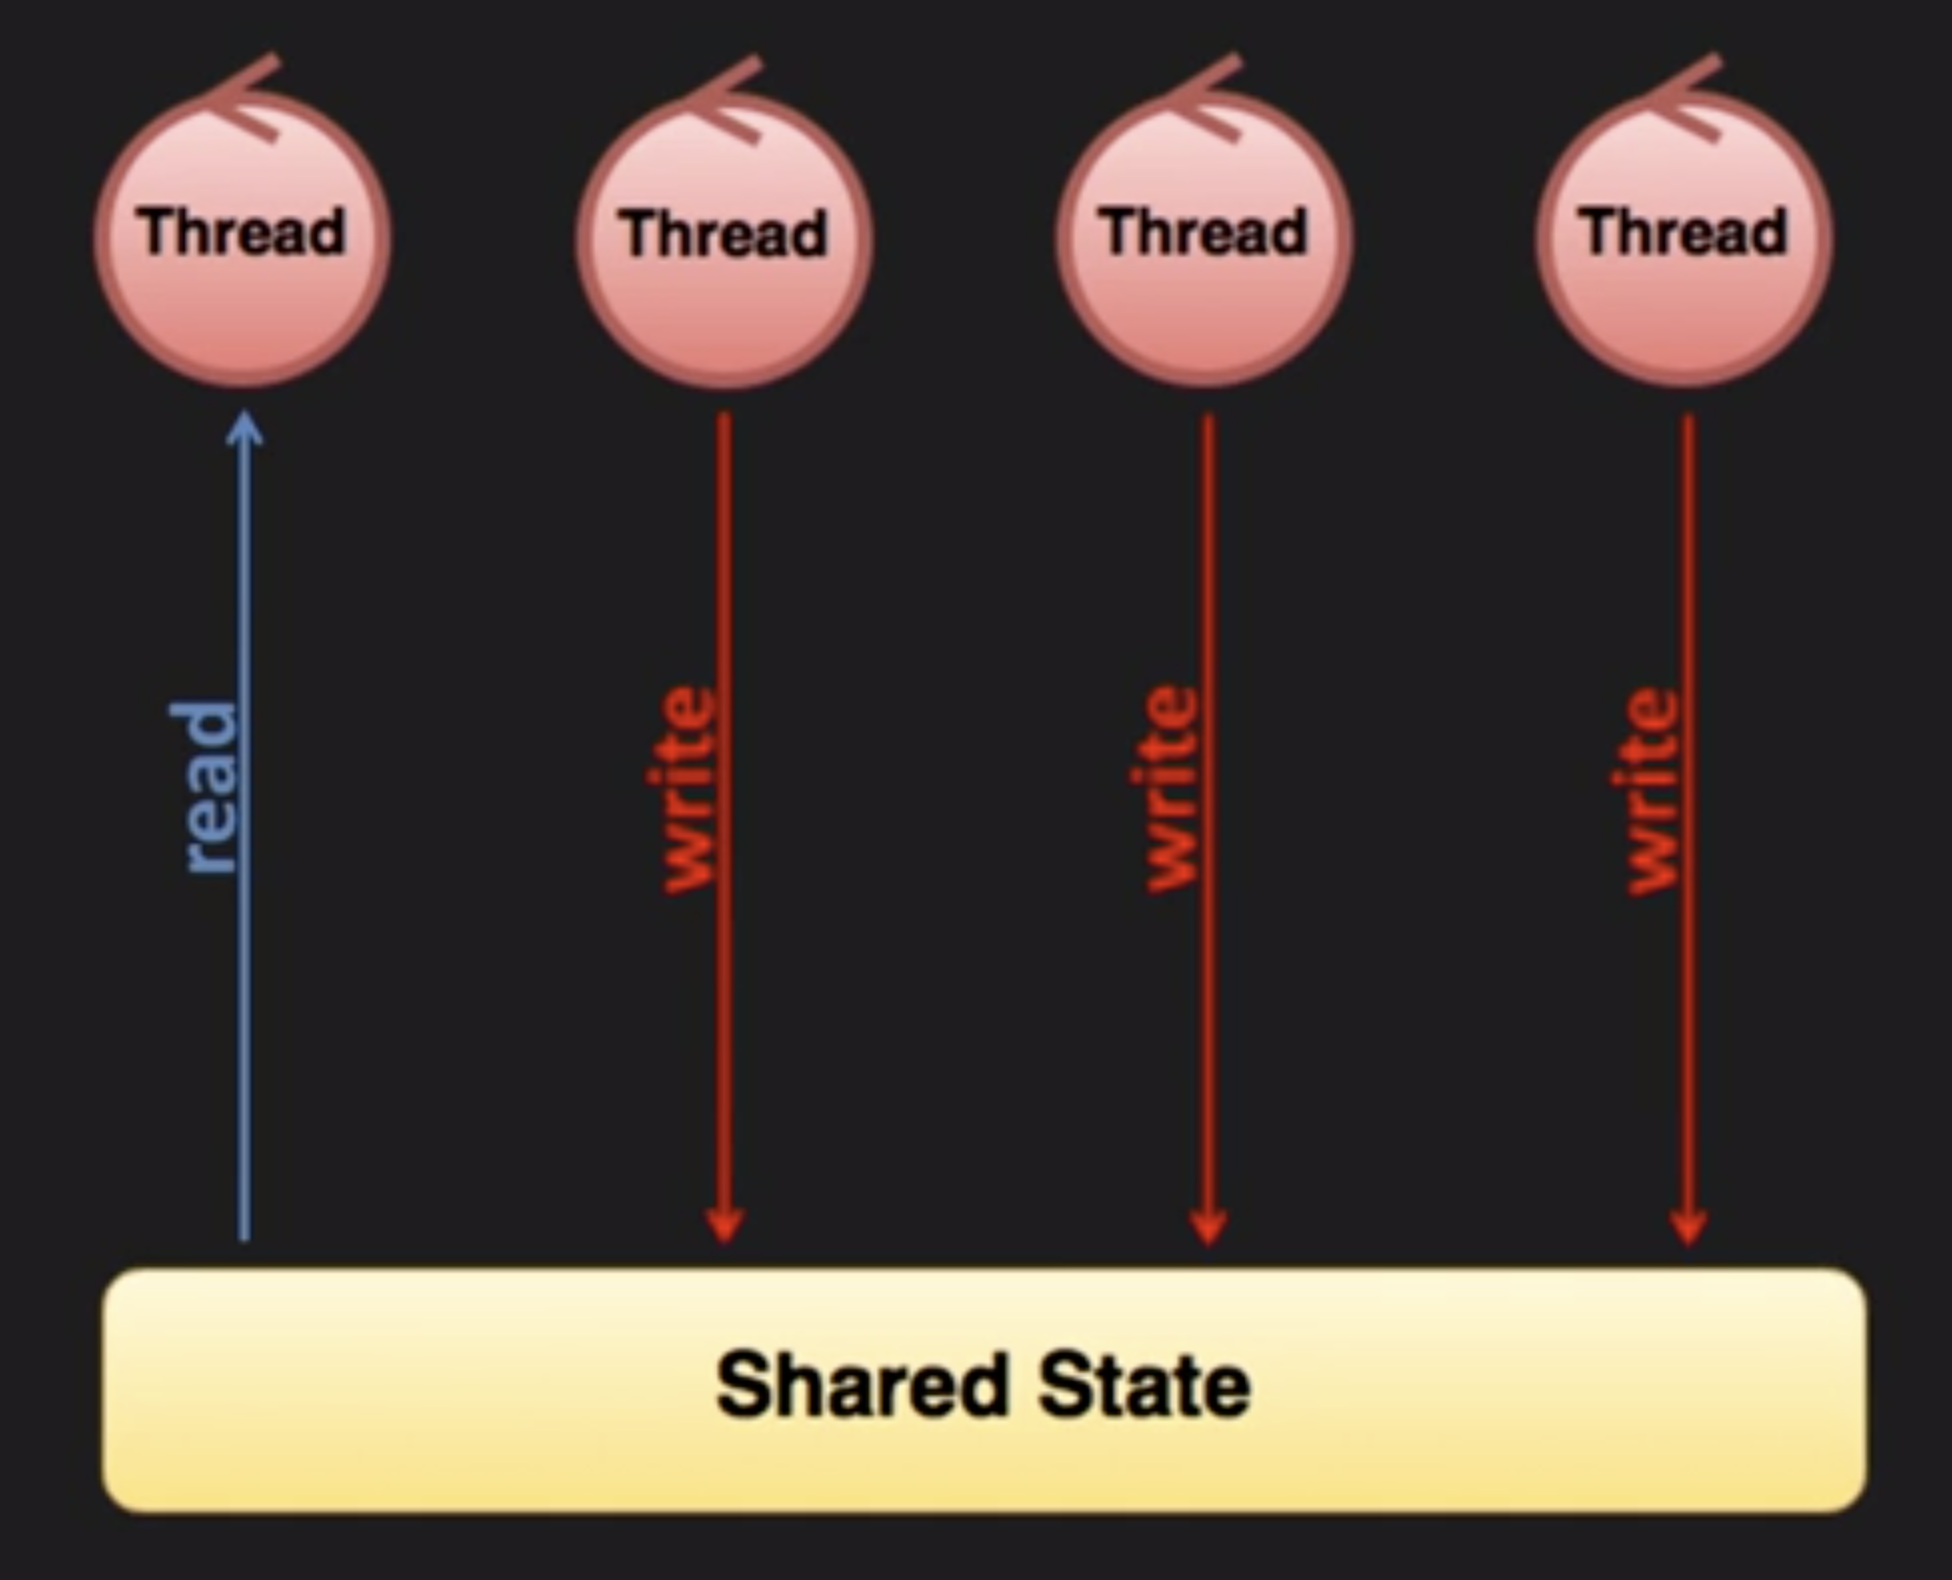
\includegraphics[width=0.75\textwidth]{images/shared}}		
\end{frame}

\begin{frame}{Synchronisation to the rescue}
\centerline{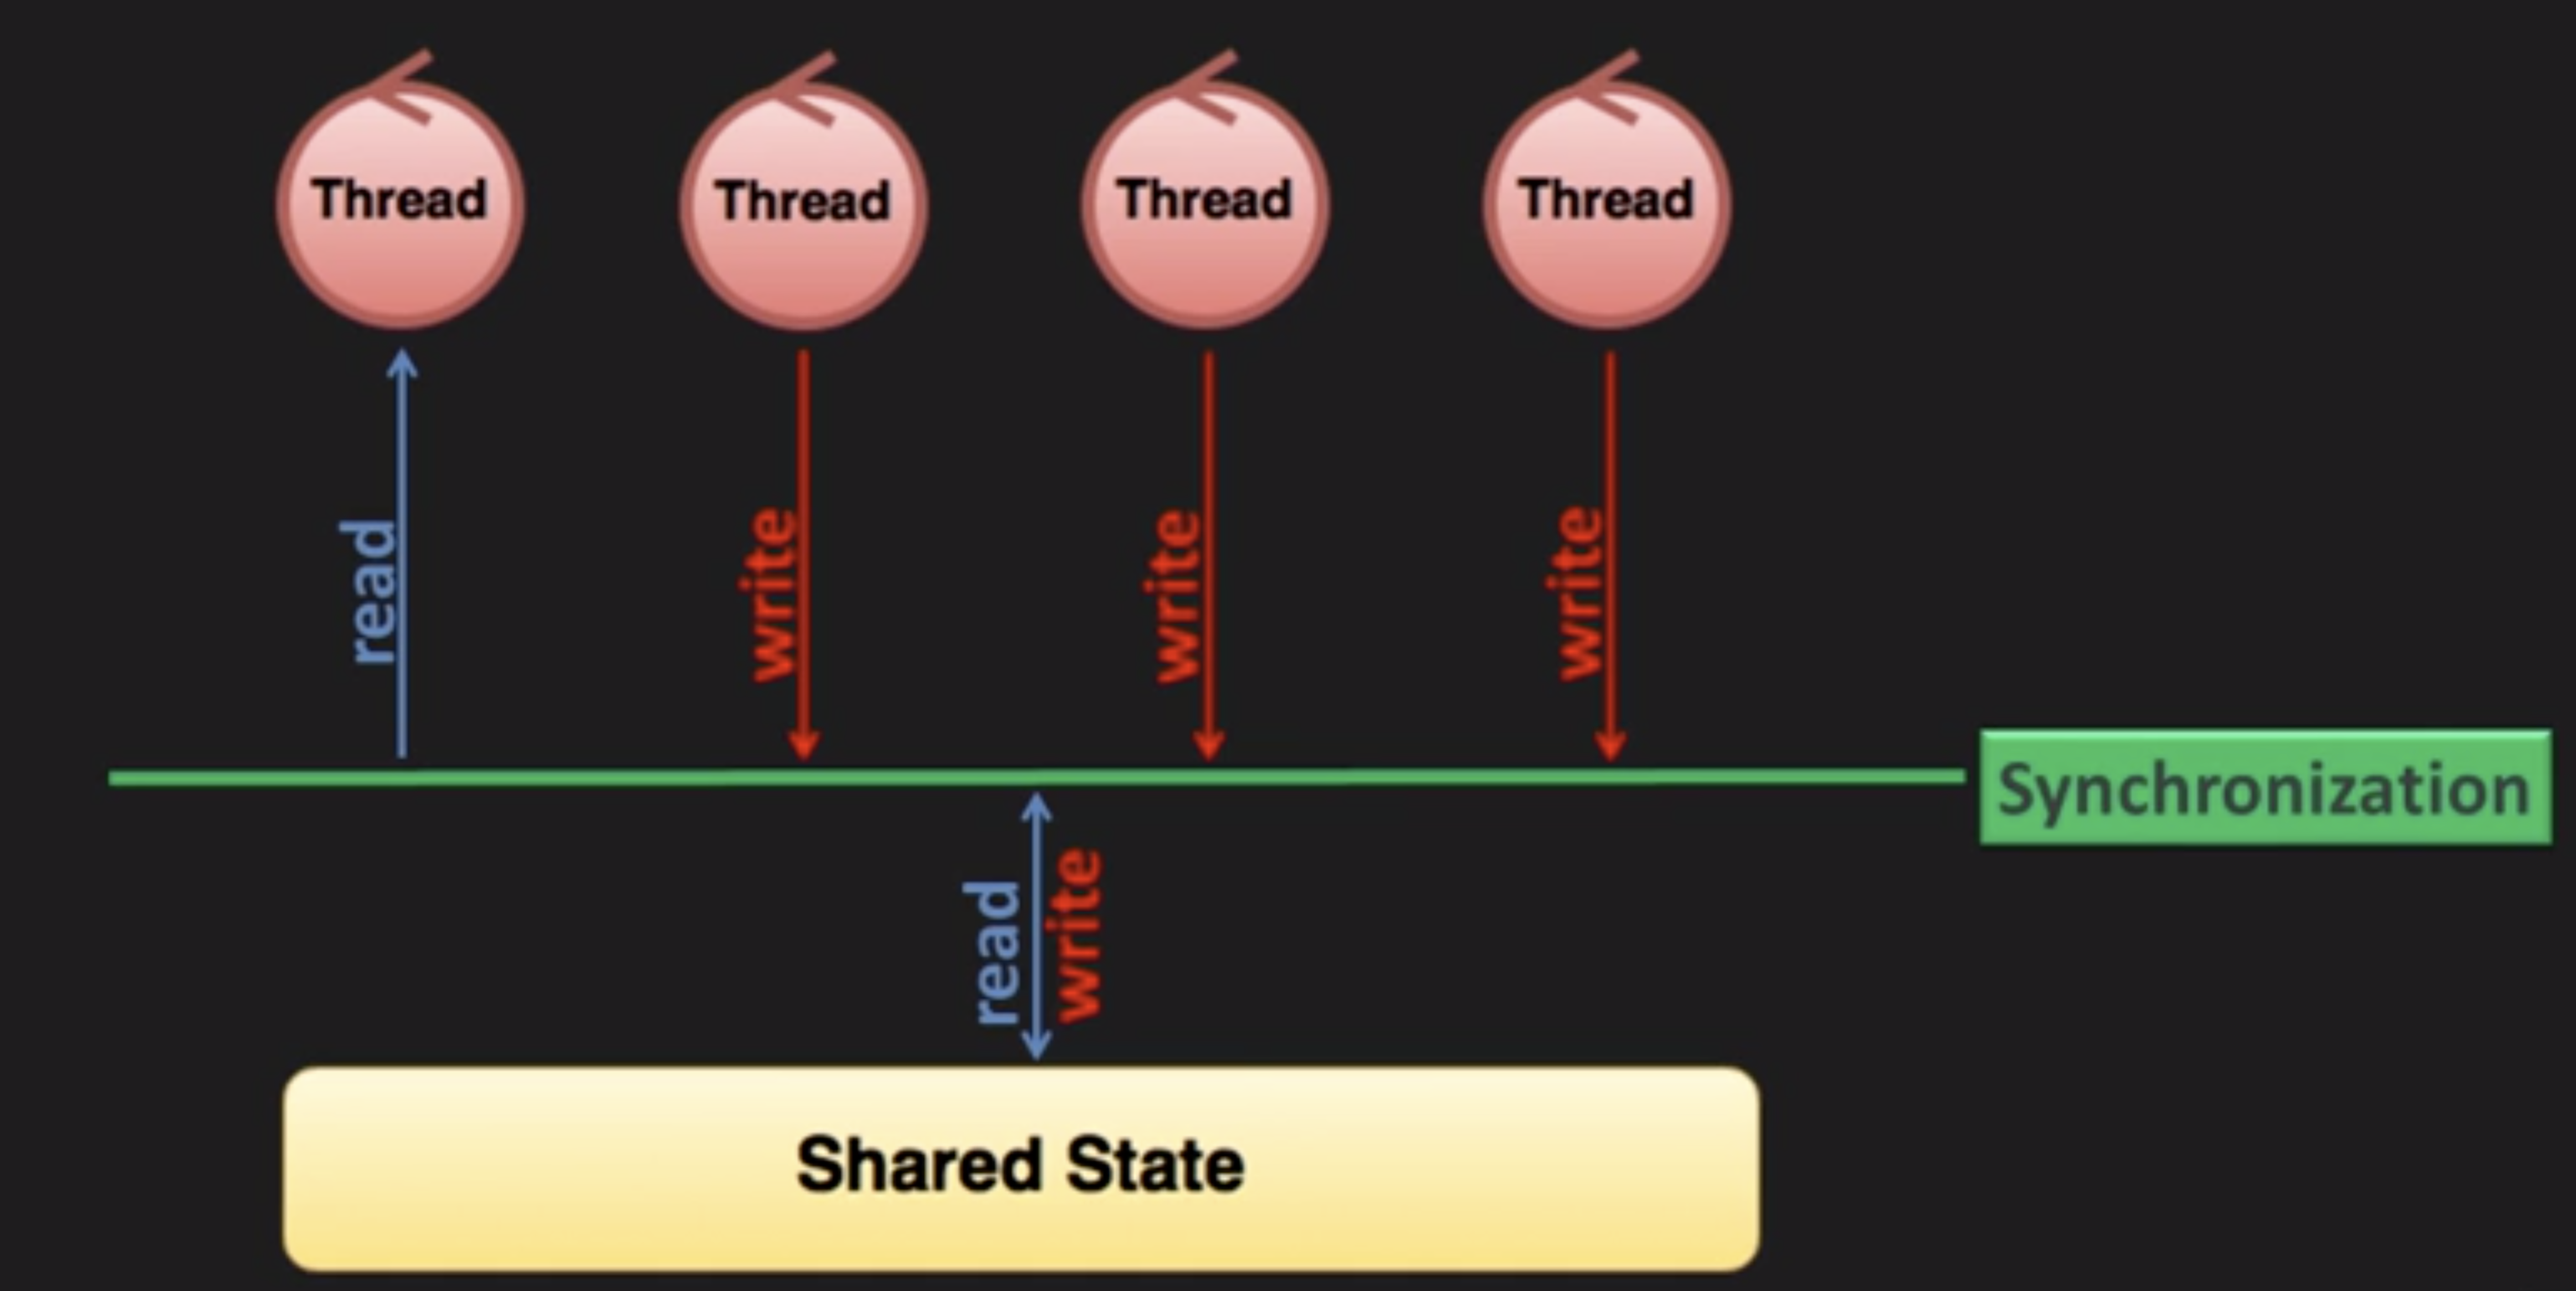
\includegraphics[width=1\textwidth]{images/sync}}		
\end{frame}

\begin{frame}{Why concurrent programming is hard	}
\begin{itemize}
\item Thread management is hard	
\item Accessing mutable shared state requires synchronisation
\item Incorrect synchronisation causes more problems than it solves
\item Issues are very difficult to reproduce and troubleshoot
\end{itemize}
	
\end{frame}

\begin{frame}{Introduction to the Actor Model}
\begin{itemize}
\item A brief history of the Actor Model
\item Actor Model fundamentals
\item Benefits and drawbacks of the Actor Model	
\end{itemize}
	
\end{frame}

\begin{frame}{A brief history of the Actor Model}
\begin{itemize}
\item The basics of the Actor Model were created and formulated by Carl Hewitt in the early 1970s
\item First major real-world implementation by Ericsson appeared in 1986 as part of the Erlang functional
programming language	
\item Akka is another implementation hosted on the JVM and, to a lesser extent, on dotNET
\end{itemize}
	
\end{frame}

\begin{frame}{Actor Model fundamentals}
\begin{itemize}
\item Everything is an Actor
\item An actor is a computational concept which is able to:
\begin{itemize}
\item react to messages it receives
\item send messages to other actors
\item create new actors
\item change its behaviour for the next message(s)	
\end{itemize}
\item It is inherently concurrent and asynchronous
\end{itemize}
	
\end{frame}

\begin{frame}{Actors}
\centerline{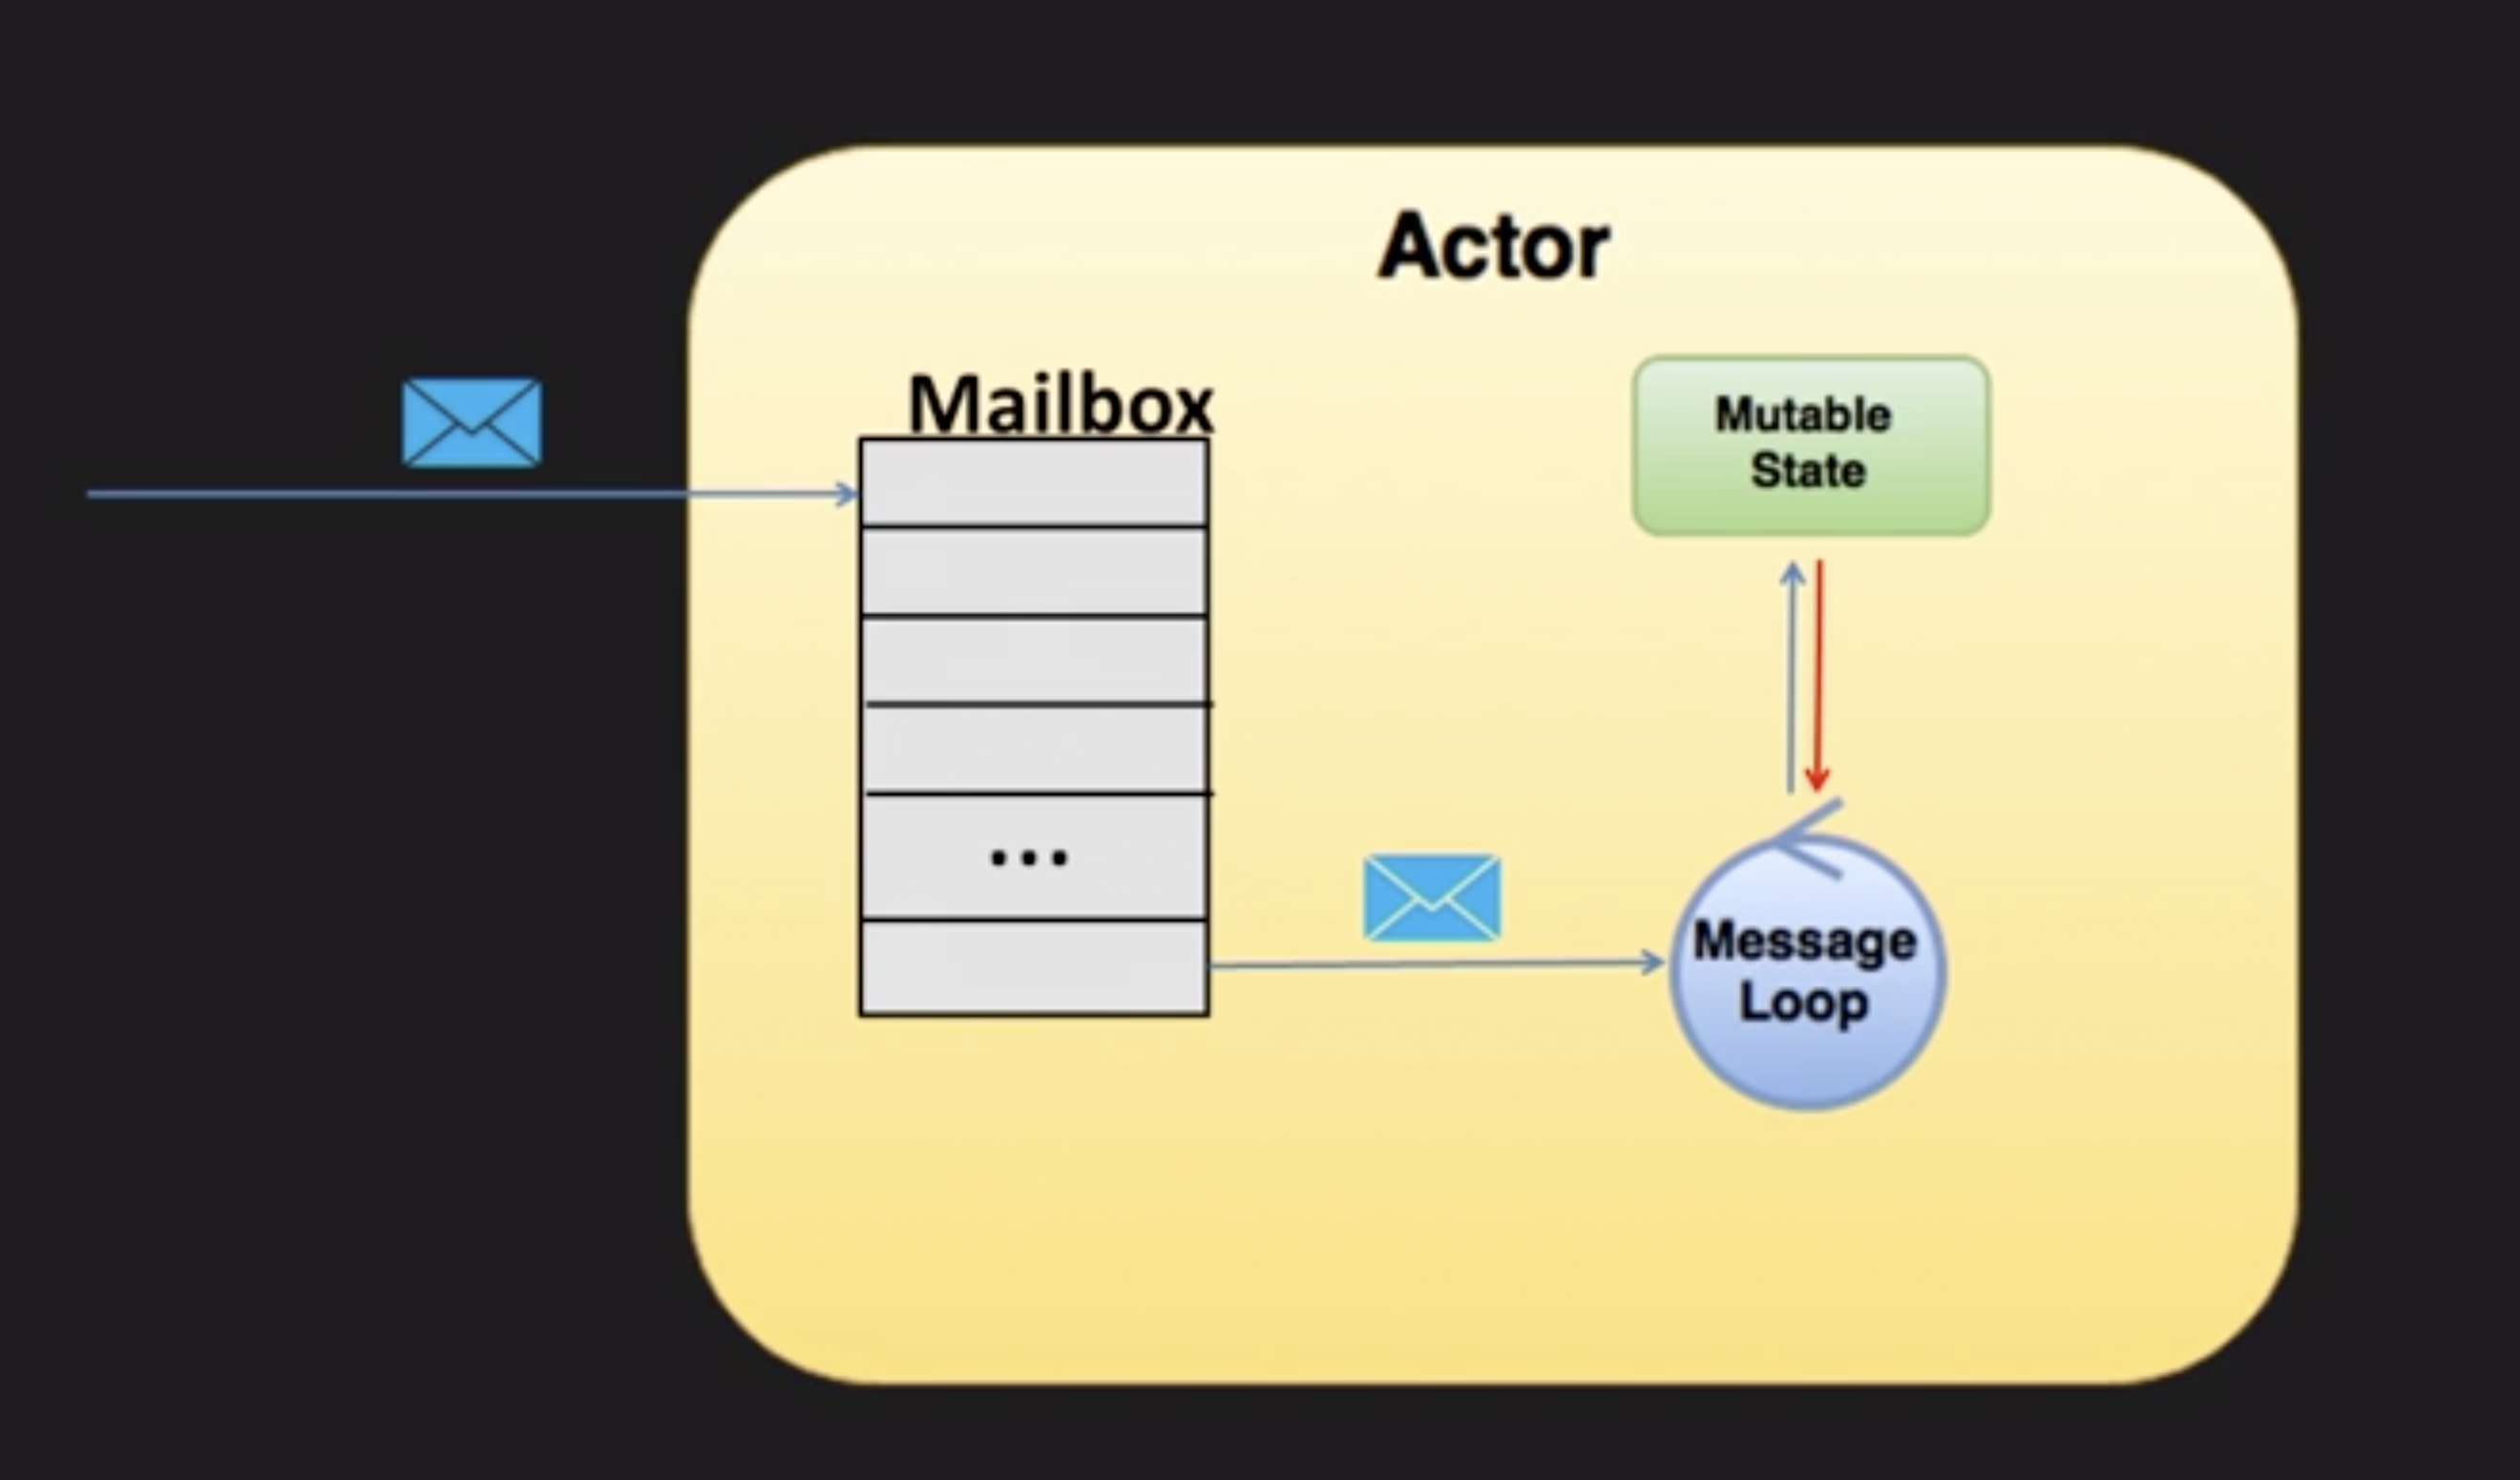
\includegraphics[width=1\textwidth]{images/actor}}		
\end{frame}

\begin{frame}{Message passing concurrency}
\centerline{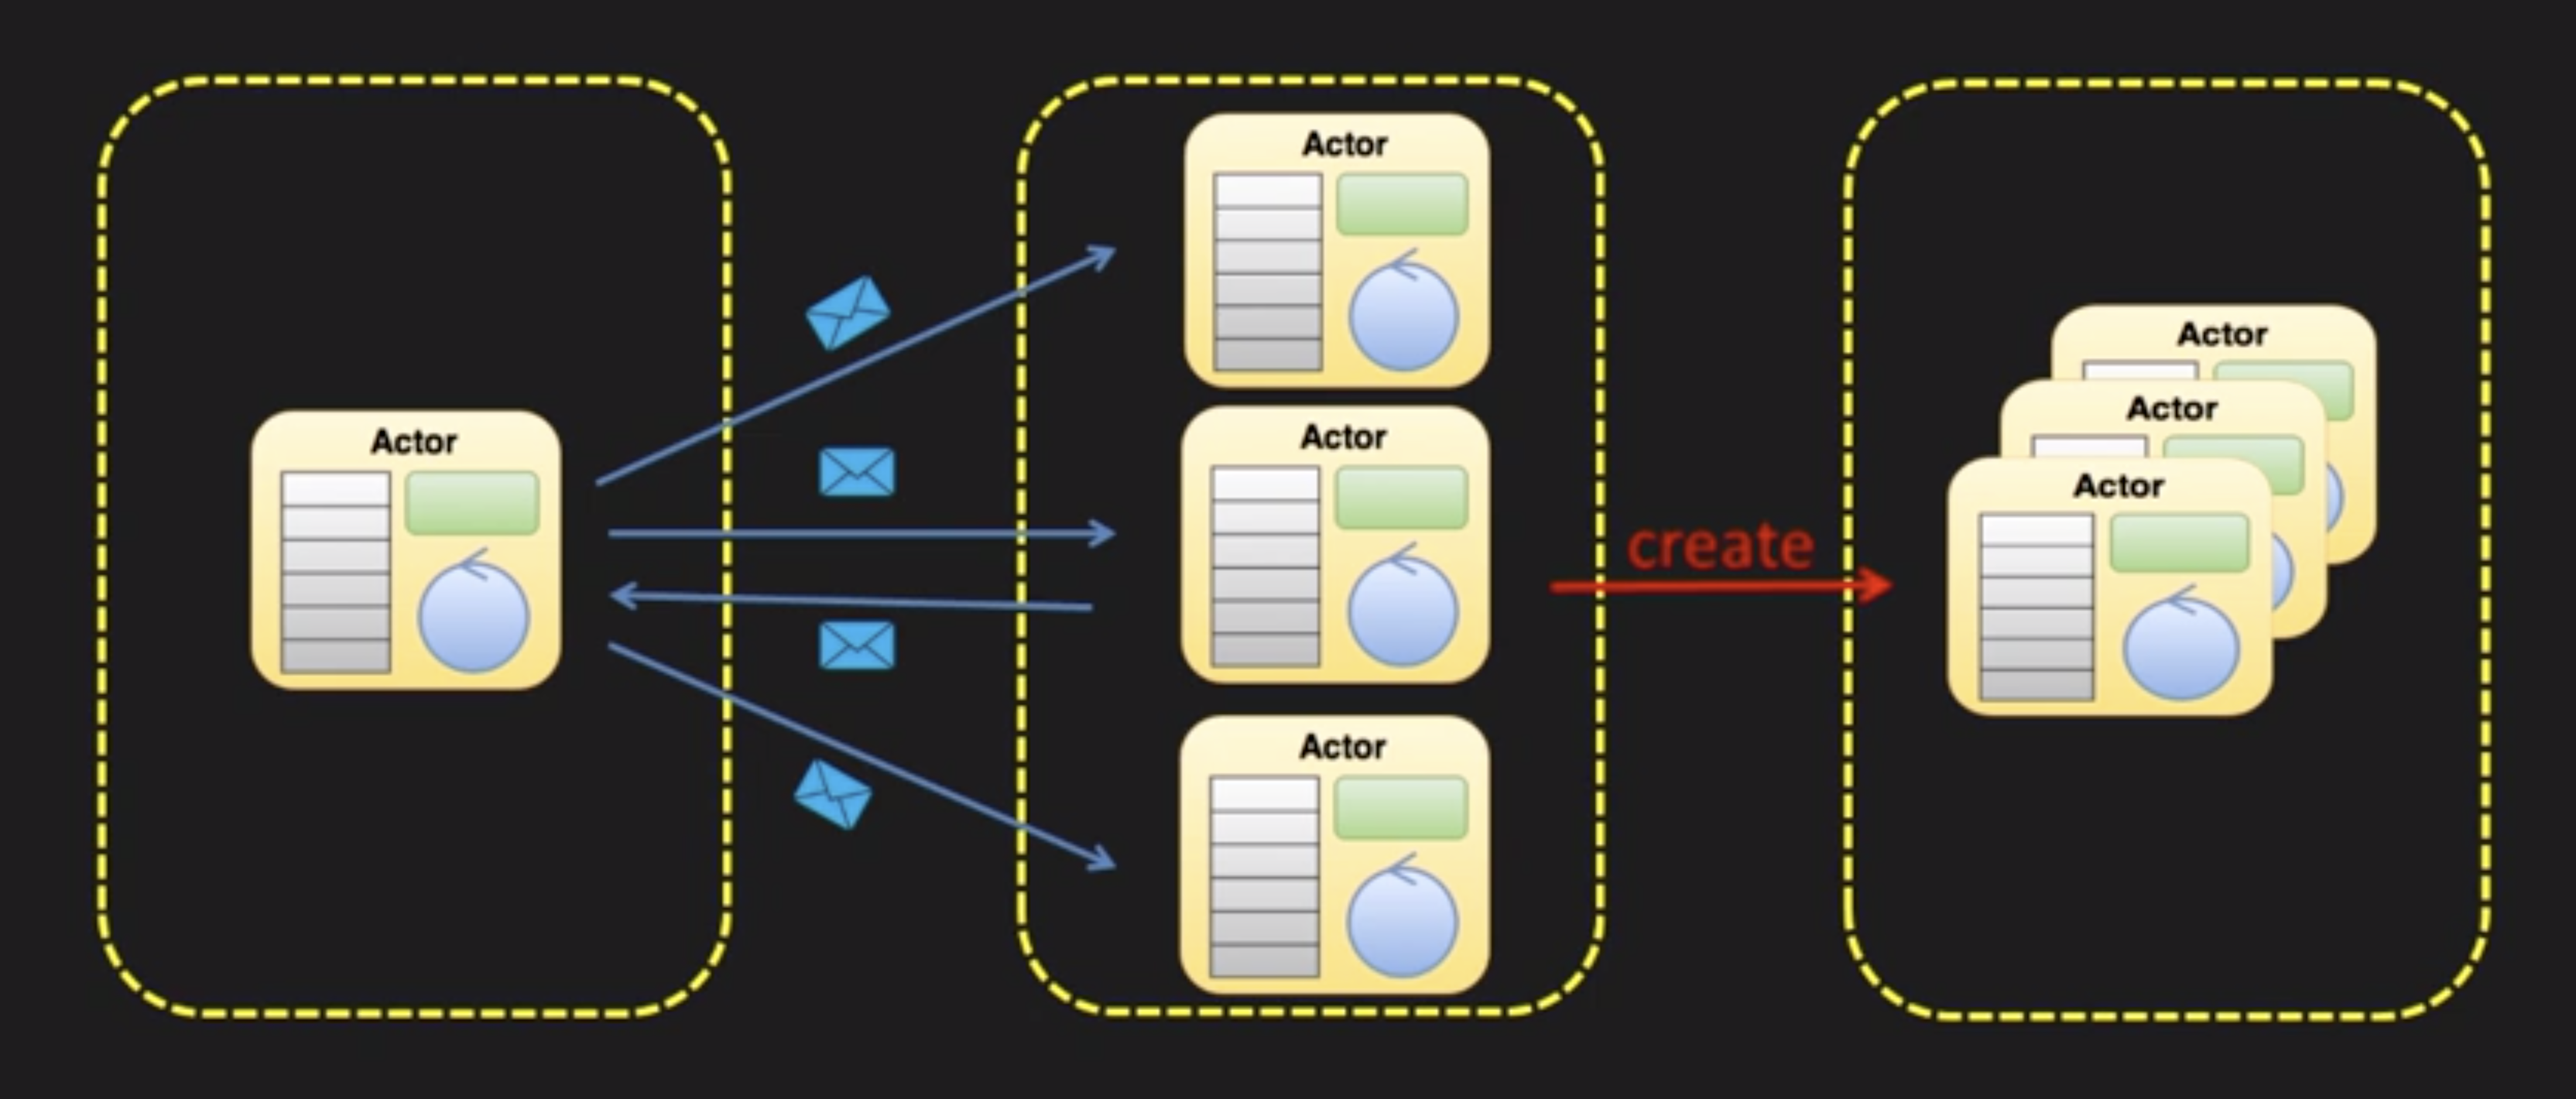
\includegraphics[width=1\textwidth]{images/message-passing}}		
\end{frame}

\begin{frame}{Benefits and drawbacks of the Actor Model}
\begin{itemize}
\item It is much simpler to reason about
\item No shared mutable state = 	no synchronisation
\item Asynchronous message passing takes some getting used to!
\item Not appropriate for every problem
\item Troubleshooting issues can be difficult
\end{itemize}
	
\end{frame}


\begin{frame}{Concurrent Programming}
\begin{itemize}
\item We are going to look at a programming language specifically designed for concurrency: \emph{Erlang}
\item Erlang is a programming language designed at the Ericsson Computer Science Laboratory
\item Erlang is a compiled concurrent functional programming language (with some roots in Prolog)
\end{itemize}
\end{frame}


\begin{frame}{Erlang}
\begin{itemize}
\item The name has two interpretations:
\begin{itemize}
\item Ericsson Language (it was originally developed at Ericsson)
\item Agner Karup Erlang was a Danish mathematician (whose work was used in telephone network analysis)
\end{itemize}
\item Open source
\item Includes extensive libraries of code for building robust fault-tolerant distributed applications
\item It has been battle tested in a number of Ericsson products, for example AXD301 (ATM switch)
\end{itemize}
\end{frame}

\begin{frame}{Akka}
\begin{itemize}
\item Jonas Boner began working on Akka in early 2009, inspired by Erlang
\item Akka was quickly adopted by the Scala community, displacing Scala's own actor model implementation
\item Akka's core is all about actors but it also has many additional modules and features	
\end{itemize}
	
\end{frame}


\begin{frame}{Erlang --- The books\ldots}

\hfill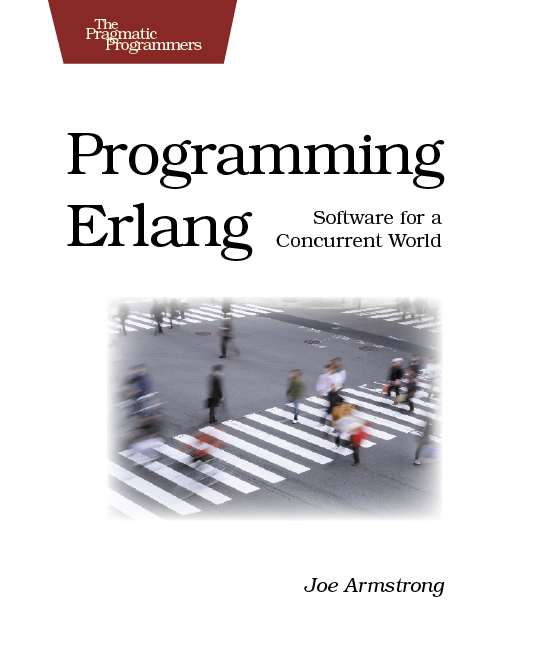
\includegraphics[width=0.4\textwidth]{images/jaerlang.png}
\hfill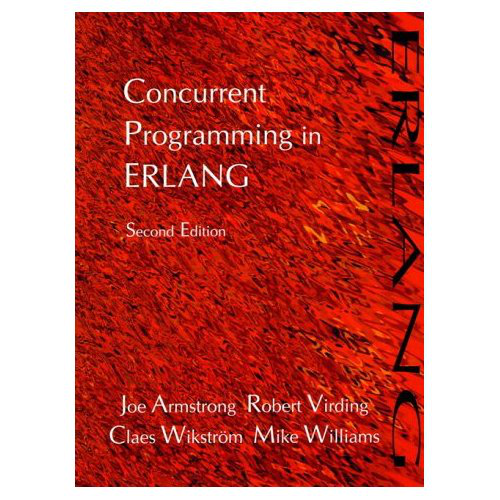
\includegraphics[width=0.4\textwidth]{images/erlang-book.png}\hfill
\end{frame}

\begin{frame}{Performance}
\begin{itemize}
\item Performance was not one of the main features of the languages we looked at so far
\item Erlang was developed with high performance in mind
\item It has to satisfy the requirements of telecom companies:
\begin{itemize}
\item Hundreds of thousands of processes have to run in a highly distributed environment
\item Processes should not be able to corrupt each other's memory
\item Systems cannot be taken down to upgrade software, i.e., hot-swapping of code has to be possible
\item Has to be able to deal with crashing processes reliably
\end{itemize}
\end{itemize}
\end{frame}

\begin{frame}{Basic Concepts}
\begin{itemize}
\item Erlang programs run on a virtual machine that automatically adapts to the underlying hardware
\begin{itemize}
\item Runs on multiple cores, multiple CPUs in a distributed system, or on a single CPU 
\end{itemize}
\item The basic building block of Erlang is a \emph{process}
\begin{itemize}
\item Can be seen as an agent running a piece of code
\item This is done concurrently to other processes, every process running at its own pace
\item Processes don't share any resources
\end{itemize}
\end{itemize}
\end{frame}

\begin{frame}{Process Communication}
\begin{itemize}
\item Sometimes processes have to interact with each other
\item This is done via message passing (i.e. copying some information and sending it to another process)
\begin{itemize}
\item This happens even if both processes are running on the same machine
\end{itemize}
\item This makes it possible to distribute Erlang applications quite easily
\item Has the downside that things that are simple to formulate in other languages are a bit harder in Erlang
\item As a programmer you have to start thinking in terms of concurrent processes
\end{itemize}
\end{frame}

\begin{frame}{Fault Tolerance}
\begin{itemize}
\item Rather than trying to achieve perfect error handling, Erlang follows the philosophy of ``Let it crash''
\item Part of the system goes down in a controlled way and then is restarted from a clean slate
\item The event leading to a crash and the crash are logged, so this can be analysed to find a possible fault
\end{itemize}
\end{frame}

\begin{frame}[fragile,allowframebreaks]{Functional Programming}
\begin{itemize}
\item Erlang is not a ``pure'' functional language, but borrows a couple of concepts from functional programming
\item In many senses Erlang was an early example of a \emph{polyglot} programming language
\item We will not go too deeply right here, only cover what we need to introduce Erlang
as we have already covered functional programming (FP) in Racket
\end{itemize}

\framebreak

For this lecture we will interpret FP to mean
\begin{itemize}
\item Programs built entirely out of functions, no objects anywhere
\item Functions will (usually) return the same values, given the same inputs
\item Functions will not (usually) have side effects, i.e., they don't modify program state
\item A variable can only be assigned a value once
\end{itemize}
\end{frame}

\begin{frame}[fragile,allowframebreaks]{First Steps in Erlang}
\begin{itemize}
\item Here's the obligatory ``Hello World!'' program in Erlang (note the period at the end):
\begin{Verbatim}
> io:format("Hello World!\n").
Hello World!
ok
\end{Verbatim}
\item Although most programs will be compiled, we'll start out with the interactive Erlang shell (like the REPL in Racket)
\item Erlang knows the standard data types:
\begin{Verbatim}
> 2 + 2.
4
> 2 + 2.0.
4.0
> "string".
"string"
\end{Verbatim}
\end{itemize}

\framebreak

\begin{itemize}
\item Erlang knows lists:
\begin{Verbatim}
> [1,2,3].
[1,2,3]
> [72,97,32,72,97,32,72,97].   
"Ha Ha Ha"
\end{Verbatim}
\item It has strong typing:
\begin{Verbatim}
> 4 + "string".
** exception error: 
   bad argument in an arithmetic expression
\end{Verbatim}
\end{itemize}

\framebreak

\begin{itemize}
\item Here are some more similarities with Prolog
\begin{Verbatim}
> variable = 4.
** exception error: no match of right hand...
> Variable = 4.
4
\end{Verbatim}
\item \texttt{variable} is an \emph{atom}, starting with a lower-case letter
\item Variables have to start with an upper-case letter
\begin{Verbatim}
> Var = 1.
1
> Var = 2.
** exception error: no match of right hand...
\end{Verbatim}
\item Variables can only be instantiated once
\end{itemize}
\end{frame}

\begin{frame}[fragile]{Tuples}
\begin{itemize}
\item Tuples are fixed-length (heterogeneous) lists
\begin{Verbatim}
> Origin = {0,0,"null point"}.
{0,0,"null point"}
\end{Verbatim}
\item In Erlang tuples are often used as maps or hashes:
\begin{Verbatim}
> {comic,{name,"Calvin & Hobbes"},
         {character,"Calvin"}}.
{comic,{name,"Calvin & Hobbes"},
       {character,"Calvin"}}
\end{Verbatim}
\item Atoms are used for the hash keys and (in this case) strings for the values
\end{itemize}
\end{frame}

\begin{frame}[fragile,allowframebreaks]{Pattern Matching}
\begin{itemize}
\item The \texttt{=} operator in Erlang isn't actually an assignment, it's a match operator
\item It can also be used on more complex structures:
\begin{Verbatim}
> Comic = {comic,{name,"Calvin & Hobbes"},
>          {character,"Calvin"}}.
{comic,{name,"Calvin & Hobbes"},
       {character,"Calvin"}}
> {comic,{name,N},{character,C}} = Comic.
{comic,{name,"Calvin & Hobbes"},
       {character,"Calvin"}}
> N.
"Calvin & Hobbes"
> C.
"Calvin"
\end{Verbatim}
\end{itemize}

\framebreak

\begin{itemize}
\item Pattern matching can also be applied to lists with head and tail elements
\begin{Verbatim}
> [Head|Tail] = [1,2,3,4].
[1,2,3,4]
> Head.
1
> Tail.
[2,3,4]
\end{Verbatim}
\item Erlang is slightly different to Prolog, in that it will not do an exhaustive search to match all possible values
\item A match will work against a single value
\item \ldots but more of that later
\end{itemize}
\end{frame}

\begin{frame}[fragile,allowframebreaks]{Modules}
\begin{itemize}
\item Code can (should?) be organised in \emph{modules}
\item Each module has a unique name consisting of an atom
\item The standard library has a lot of predefined modules, e.g. the \texttt{lists} module to work with lists
\item When calling a function from another module you need a qualified name
\begin{Verbatim}
> lists:reverse([1,2,3,4]).
[4,3,2,1]
\end{Verbatim}
\item You've already seen the module \texttt{io} for printing ``Hello World!''
\end{itemize}

\framebreak

To create your own module, you need to do the following:
\begin{enumerate}
\item Write a source file
\item Compile it
\item Load it
\end{enumerate}
Let's do this for a very simple piece of code:
\begin{itemize}
\item A function that returns its input value
\end{itemize}

\framebreak

\begin{itemize}
\item This is what the module file \texttt{basic.erl} looks like:
\begin{Verbatim}
-module(basic).
-export([mirror/1]).

mirror(Anything) -> Anything.
\end{Verbatim}
\item The first line defines the name of the module
\item The second line tells Erlang that the function \texttt{mirror} 
\begin{itemize}
\item should be visible outside of the module
\item has one parameter (that is the meaning of \texttt{/1})
\end{itemize}
\item Finally, the function itself is defined
\end{itemize}

\framebreak

\begin{itemize}
\item Next you have to compile the file
\item Start the Erlang shell from the directory of the code file and compile it
\begin{Verbatim}
> c(basic).
{ok,basic}
\end{Verbatim}
\item Now you can run it (as you can see, Erlang is dynamically typed):
\begin{Verbatim}
> basic:mirror(1).
1
> basic:mirror(xxx).
xxx
> basic:mirror("string").
"string"
\end{Verbatim}
\end{itemize}

\framebreak

\begin{itemize}
\item Let's have a look at yet another module with multiple matching possibilities
\begin{Verbatim}
-module(yam).
-export([fac/1]).
-export([fib/1]).

fac(0) -> 1;
fac(N) -> N * fac(N-1).

fib(0) -> 1;
fib(1) -> 1;
fib(N) -> fib(N-1) + fib(N-2).
\end{Verbatim}
\end{itemize}

\framebreak

\begin{itemize}
\item Each possible match has
\begin{itemize}
\item the function name
\item the argument to match
\item the code to execute after the \texttt{->} symbol
\end{itemize}
\item The last statement is terminated with \texttt{.} and all others with \texttt{;}
\item Control structures, which we will look at next, have a similar structure
\end{itemize}
\end{frame}

\begin{frame}[fragile,allowframebreaks]{Control Structures}
\begin{itemize}
\item The \emph{case} statement in Erlang looks like this:
\begin{Verbatim}
> Animal = "dog".
"dog"
> case Animal of
>    "dog" -> underdog;
>    "cat" -> thundercat;
>    "elephant" -> dumbo;
>    _ -> something_else
> end.
underdog
\end{Verbatim}
\item The underscore \texttt{\_} matches anything
\end{itemize}

\framebreak

\begin{itemize}
\item One of the branches of a \texttt{case} or \texttt{if} statement has to be true
\begin{Verbatim}
> if   
>    X > 0 -> positive;
>    X < 0 -> negative;
>    true  -> zero
> end.
\end{Verbatim}
\end{itemize}
\end{frame}

\begin{frame}[fragile,allowframebreaks]{Anonymous Functions}
A function that returns functions or takes functions as arguments is called a \emph{higher-order function}
(Yes, we know that!@!)
\begin{itemize}
\item In Ruby this was achieved using code blocks
\item In Erlang arbitrary functions can be assigned to variables and be passed around like any other data type
\end{itemize}

\framebreak

\begin{itemize}
\item Let's define a function that negates its argument
\begin{Verbatim}
> Negate = fun(I) -> -I end.
#Fun<erl_eval.6.111823515>
> Negate(1).
-1
> Negate(-3).
3
\end{Verbatim}
\item The keyword \texttt{fun} defines an anonymous function
\item This function is assigned to \texttt{Negate}
\item \texttt{Negate} actually \emph{is} the function, not just the value returned by the function
\end{itemize}
\end{frame}

\begin{frame}[fragile,allowframebreaks]{Lists and Higher-order Functions}
\begin{itemize}
\item Together with lists, higher-order functions can achieve some interesting things
\item We'll have a closer look at the module \texttt{lists} now
\item \texttt{lists:foreach} takes a function and a list as arguments and iterates over the list applying the function
\begin{Verbatim}
> Numbers = [1,2,3,4].
> Print = fun(X) -> io:format("~p~n", [X]) end.
> lists:foreach(Print,Numbers).
1
2
3
4
ok
\end{Verbatim}
\end{itemize}

\framebreak

\begin{itemize}
\item The \texttt{map} function also takes a function and a list
\item However, it applies the function to each element and builds a list with the results
\begin{Verbatim}
> lists:map(fun(X) -> X+1 end,Numbers).
[2,3,4,5]
\end{Verbatim}
\item Lists can also be filtered:
\begin{Verbatim}
> Small = fun(X) -> X < 3 end.
> Small(4).
false
> Small(2).
true
lists:filter(Small,Numbers).
[1,2]
\end{Verbatim}
\end{itemize}
\end{frame}

\begin{frame}[fragile]{Fold functions}
\begin{itemize}
\item \emph{Fold} functions are a family of functions that accumulate a return value while processing a data structure
\item A fold function takes a function, an initial accumulator value, and a list
\begin{Verbatim}
> Adder = fun(Item,TmpSum) -> Item+TmpSum end.
> InitSum = 0.
> lists:foldl(Adder,InitSum,Numbers).
10
\end{Verbatim}
\item Fold functions for lists come in two flavours: \texttt{foldl} and \texttt{foldr}
\end{itemize}
\end{frame}

\begin{frame}{\texttt{foldl} vs \texttt{foldr}}
\begin{itemize}
\item Both of them take the same parameters: a function, initial accumulator value, and a list
\item The difference is the order in which they combine the list elements with the accumulator
\item \texttt{foldl} accumulates elements from left to right
\item \texttt{foldr} accumulates elements from right to left
\end{itemize}
\end{frame}

\begin{frame}
\centerline{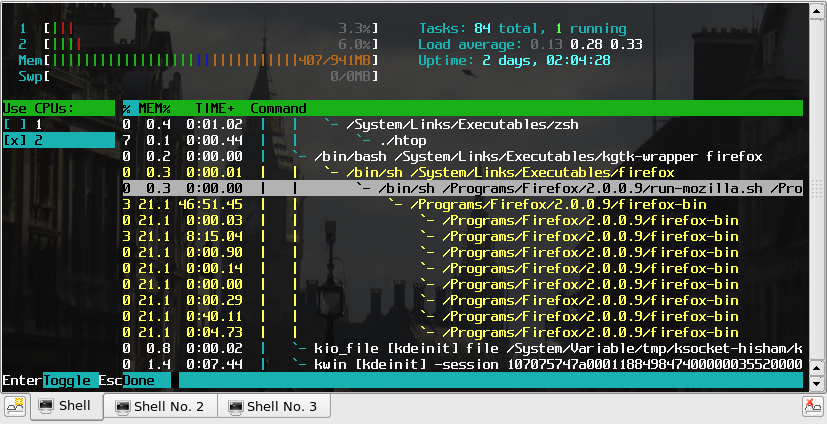
\includegraphics[width=\textwidth]{images/processes.png}}
\centerline{\Huge\textbf{Processes!}}
\end{frame}

\begin{frame}[fragile,allowframebreaks]{Processes}
\begin{itemize}
\item Processes are the fundamental units of concurrency in Erlang
\item They communicate with each other via messages
\item Processes are also the basic container for program state in Erlang
\item Now let's see what we can do with processes
\end{itemize}

\framebreak

\begin{itemize}
\item Three basic primitives for processes are
\begin{itemize}
\item sending a message (with \texttt{!}, pronounced ``bang'')
\item creating a new process (with \texttt{spawn})
\item receiving a message (with \texttt{receive})
\end{itemize}
\item That's enough to get us started
\item Let's write a simple translation process that gets a word in Spanish and replies with an English translation
(BTW --- I don't know these languages but that doesn't matter)
\end{itemize}
\end{frame}

\begin{frame}[fragile,allowframebreaks]{Lost in Translation}

\centerline{
\includegraphics[scale=0.6]{images/Lost_in_Translation_poster.png}}

\framebreak

\begin{Verbatim}
-module(translate).
-export([loop/0]).
loop() ->
  receive
    "casa" -> 
      io:format("house~n"),
      loop();
    "blanca" -> 
      io:format("white~n"),
      loop();
    _ ->
      io:format("?~n"),
      loop()
  end.
\end{Verbatim}
\end{frame}

\begin{frame}[fragile]{Translation Process}
\begin{itemize}
\item We start out with a function \texttt{loop} that calls \texttt{receive}, which works similar to 
a \texttt{case} statement
\begin{Verbatim}
loop() ->
  receive
    ...
  end.
\end{Verbatim}
\item \texttt{receive} will try to match a received message to one of the clauses
\item If statements in a matching clause span more than one line, they are separated by commas
\item All clauses display something and then call \texttt{loop}, resulting in an endless recursion/loop
\end{itemize}
\end{frame}

\begin{frame}[fragile]{Running the Process}
\begin{itemize}
\item After compiling the module \texttt{translate} we can create a process running the function \texttt{loop}
\begin{Verbatim}
> Pid = spawn(fun translate:loop/0).
<0.130.0>
\end{Verbatim}
\item Now we have the process (with ID 0.130.0) up and running
\item However, it's not doing much: it's just sitting there waiting for messages
\end{itemize}
\end{frame}

\begin{frame}[fragile]{Sending Messages}
\begin{itemize}
\item So we should send some messages to it (with the \texttt{!} operator)
\begin{Verbatim}
> Pid ! "casa".
house
"casa"
> Pid ! "blanca".
white
"blanca"
> Pid ! "loco".  
?
"loco"
\end{Verbatim}
\end{itemize}
\end{frame}

\begin{frame}[fragile]{Variations on Processes}
\begin{itemize}
\item You can also spawn processes on a remote machine using a slightly different syntax:
\begin{Verbatim}
spawn(Node,function).
\end{Verbatim}
\item It is also possible to send messages to processes running on other nodes
\begin{Verbatim}
node@server ! message
\end{Verbatim}
\end{itemize}
\end{frame}

\begin{frame}{Messaging}
\begin{itemize}
\item What we've just implemented is called asynchronous messaging
\item The sender sends a message, but does not wait actively for a reply
\begin{itemize}
\item E-mails and SMS text messages are asynchronous
\end{itemize}
\item In synchronous messaging, the sender sends a message and actively waits for the response
\begin{itemize}
\item Phone calls and loading a web page are synchronous 
\end{itemize}
\end{itemize}
\end{frame}

\begin{frame}[fragile,allowframebreaks]{Synchronous Messaging}
To change the translation service to synchronous messaging we need to do the following
\begin{itemize}
\item Instead of printing the result, each \texttt{receive} clause has to send a response
\item In addition to the word to translate, each \texttt{receive} clause will also need the ID of the sender
\item On the sender side, instead of using \texttt{!}, we'll write a 
simple function sending a request and waiting for the response
\end{itemize}

\framebreak

\begin{itemize}
\item For the first two points, we need to rewrite the \texttt{receive} clauses
\begin{Verbatim}
receive
  ...
  {Pid,"xxx"} ->
    Pid ! "yyy",
    loop();
  ...
\end{Verbatim}
\item Instead of just matching the message, we also match the ID of the sender (in a tuple)
\item Also, instead of printing the result, we send it to a process
\end{itemize}

\framebreak

\begin{itemize}
\item Starting a process with the new modified \texttt{loop} function and sending something to it is not enough
\begin{Verbatim}
> Trans = spawn(fun translate2:loop/0).
<0.144.0>
> Trans ! {self(),"casa"}.
{<0.61.0>,"casa"}
\end{Verbatim}
\item We send the correct tuple to the process, but we don't pick up its answer
\item Next we'll write a function that will send a message and wait for the reply
\end{itemize}

\framebreak

\begin{itemize}
\item On the sender side, we would have to run the following code
\begin{Verbatim}
translate(To,Word) ->
  To ! {self(),Word},
  receive
    Translation -> Translation
  end.
\end{Verbatim}
\item The complete module is shown on the next slide
\end{itemize}

\framebreak

\relsize{-2}
\begin{Verbatim}
-module(translate2).
-export([loop/0]).
-export([translate/2]).

loop() ->
  receive
    {Pid, "casa"} -> 
      Pid ! "house",      
      loop();
    {Pid, "blanca"} -> 
      Pid ! "white",      
      loop();
    {Pid, _} -> 
      Pid ! "?",		
      loop()			
  end.				

translate(To,Word) ->
  To ! {self(),Word},
  receive
    Translation -> Translation
  end.
\end{Verbatim}
\relsize{+2}

\framebreak

\begin{itemize}
\item After compiling it, we can spawn a process running \texttt{loop} and then 
send messages using \texttt{translate}
\begin{Verbatim}
> Trans = spawn(fun translate2:loop/0).
<0.39.0>
> translate2:translate(Trans,"blanca").
"white"
> translate2:translate(Trans,"blanca").
"white"
> translate2:translate(Trans,"xxx").   
"?"
\end{Verbatim}
\item The new version of \texttt{translate} sends a message and then waits for the reply
\end{itemize}
\end{frame}

\begin{frame}{The Downside}
\begin{columns}
\begin{column}[t]{5.5cm}

\includegraphics[width=\textwidth]{images/synccalls1.png}
\end{column}
%
\begin{column}[t]{5.5cm}
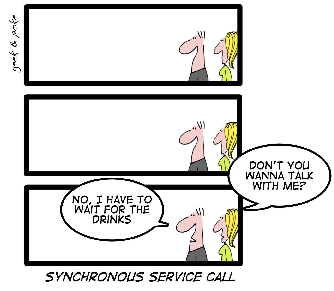
\includegraphics[width=\textwidth]{images/synccalls2.png}
\end{column}
\end{columns}
\end{frame}

\begin{frame}{Adding Reliability}
\begin{itemize}
\item Erlang has \emph{exception handling} for catching errors in a piece of code
\begin{itemize}
\item This is very similar to what Java offers, so we are not covering it here
\end{itemize}
\item In addition to this Erlang provides \emph{process links}
\begin{itemize}
\item This is a system for handling process failures
\item We are going have a closer look at process links
\end{itemize}
\end{itemize}
\end{frame}

\begin{frame}{Process Links}
\begin{itemize}
\item Whenever an Erlang process dies unexpectedly, an exit signal is generated
\item All processes linked to the dying process receive this signal
\item By default, this causes the receiver to exit as well (sending another exit signal)
\begin{itemize}
\item So you can have a whole cascade of exiting processes
\end{itemize}
\item What is the advantage of this?
\begin{itemize}
\item Allows you to have a group of processes behave as a single application
\item You don't have to worry about leftover processes still running
\end{itemize}
\end{itemize}
\end{frame}

\begin{frame}{Supervision}
\begin{itemize}
\item However, you don't always want to shut down a process when receiving an exit signal
\item Someone needs to be there to restart parts of the system when receiving exit signals
\item These \emph{supervisor processes} need to be able to override the default exiting behaviour
\item This can be done by trapping an exit signal, i.e., you get informed, but don't exit yourself
\begin{itemize}
\item Non-trapping processing are usually called \emph{worker processes}
\end{itemize}
\item Let's look at an example
\end{itemize}
\end{frame}

\begin{frame}[fragile,allowframebreaks]{Russian Roulette}

\centerline{\ldots movie clip\ldots}

\framebreak

\centerline{
\includegraphics[scale=0.4]{images/1978-walken.png}}
\framebreak

First, let's build a process that can be killed deliberately:
\begin{Verbatim}
-module(roulette).
-export([loop/0]).

loop() ->
  receive
    3 -> 
      io:format("bang!~n"),
      exit({roulette,die,at,erlang:time()});
    _ -> 
      io:format("click.~n"),
      loop()
  end.			
\end{Verbatim}

\framebreak

Let's start the process and try it out
\begin{Verbatim}
> Gun = spawn(fun roulette:loop/0).
<0.39.0>
> Gun ! 1.
click.
1
> erlang:is_process_alive(Gun).
true
>  Gun ! 3.
bang!
3
> erlang:is_process_alive(Gun).
false
\end{Verbatim}
\end{frame}

\begin{frame}[fragile,allowframebreaks]{Gun Control}
Now let's build a process that will trap exit signals:
\relsize{-1}
\begin{Verbatim}
-module(coroner).
-export([loop/0]).

loop() ->
  process_flag(trap_exit,true),
  receive
    {link,Process} ->
      link(Process),
      io:format("Supervising new process.~n"),
      loop();
    {'EXIT',From,Reason} ->
      io:format("~p died: ~p~n",[From,Reason]),
      io:format("Please start another one.~n"),
      loop();
    _ ->
      io:format("Unexpected message received.~n"),
      loop()	
  end.		
\end{Verbatim}
\relsize{+1}

\framebreak
\relsize{-1}
\begin{Verbatim}
> c(coroner).
{ok,coroner}
> c(roulette).
{ok,roulette}
> Coroner=spawn(fun coroner:loop/0).
<0.44.0>
> Gun=spawn(fun roulette:loop/0).
<0.46.0>
>  Coroner ! {link,Gun}.
Supervising new process.
{link,<0.46.0>}
> Gun ! 3.
bang!
3
<0.46.0> died: {roulette,die,at,{14,42,57}}
Please start another one.
\end{Verbatim}
\relsize{+1}
\end{frame}

\begin{frame}{Coroner}
\begin{itemize}
\item The module \texttt{coroner} does not do much at this point
\item It only notices that the \texttt{roulette} process dies
\item We are going to improve the module by
\begin{itemize}
\item moving the creation of a new \texttt{roulette} process into this new process
\item automatically re-spawning a new \texttt{roulette} process if it gets killed
\item registering the \texttt{roulette} process ID with an atom called \texttt{gun}
so that a user does not have to remember the PID to play
\end{itemize}
\end{itemize}
\end{frame}

\begin{frame}[fragile,allowframebreaks]{Meet the Doctor}

\relsize{-1}
\begin{Verbatim}
-module(doctor).
-export([loop/0]).

loop() ->
  process_flag(trap_exit,true),
  receive
    new ->
      io:format("Creating and supervising new process.~n"),
      register(gun,spawn_link(fun roulette:loop/0)),
      loop();
    {'EXIT',From,Reason} ->
      io:format("~p died: ~p~n",[From,Reason]),
      io:format("Restarting.~n"),
      self() ! new,
      loop();
    _ ->
      io:format("Unexpected message received.~n"),
      loop()	
  end.		
\end{Verbatim}
\relsize{+1}

\framebreak

\begin{itemize}
\item With \texttt{spawn\_link} we create a new process and (atomically) link it to the calling process
\item \texttt{register(gun,...)} binds the PID returned by \verb!spawn_link! to the atom \texttt{gun}
\item For restarting a \texttt{roulette} process, the \texttt{doctor} process 
just sends the message \texttt{new} to itself
\item Let's have a look
\end{itemize}

\framebreak

\relsize{-2}
\begin{Verbatim}
> c(roulette).
{ok,roulette}
> c(doctor).
{ok,doctor}
> Doc=spawn(fun doctor:loop/0).
<0.44.0>
> Doc ! new.
Creating and supervising new process.
new
> gun ! 1.
click.
1
> gun ! 3.
bang!
3
<0.48.0> died: {roulette,die,at,{15,0,32}}
Restarting.
Creating and supervising new process.
> gun ! 1.
click.
1
\end{Verbatim}
\relsize{+2}
\end{frame}

\begin{frame}[fragile,allowframebreaks]{Managing Subsystems}
\begin{itemize}
\item Usually a supervisor monitors more than one process
\item Typically it manages different groups of processes
\item These subsystems can then be cleanly restarted
\item On the right hand side, one of the processes in the left subgroup crashes\dots
\item \dots the whole subgroup is terminated and restarted
\end{itemize}

\framebreak

\begin{center}
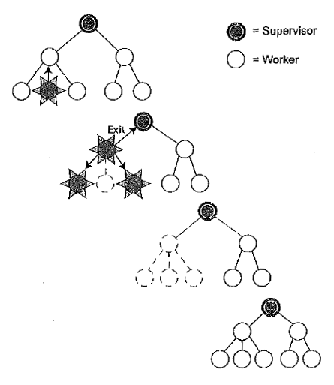
\includegraphics[scale=.55]{images/supervisor1.png}
\end{center}

\framebreak

\begin{itemize}
\item Usually you should build a whole \emph{supervision tree} with multiple layers of supervisors
\item This gives you a finer granularity in terms of ``rebooting'' certain parts of the system
\end{itemize}

\begin{center}
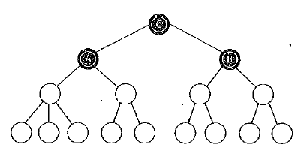
\includegraphics[scale=.65]{images/supervisor2.png}
\end{center}
\end{frame}

\begin{frame}{Open Telecom Platform}
\begin{itemize}
\item We have only been able to cover a small part of Erlang
\item The Open Telecom Platform (OTP) is a powerful package that helps Erlang reach its full potential
\item It's not specific to telecom applications and helps in
\begin{itemize}
\item writing stable and reliable code (OTP has been thoroughly used and tested)
\item providing frameworks for applications
\item offering functionality for code upgrades
\end{itemize}
\end{itemize}
\end{frame}

\begin{frame}{Summary --- Strengths of Erlang}
\begin{itemize}
\item Erlang offers a lot in terms of concurrency, performance, reliability, and fault tolerance
\item The share-nothing, message-passing process model is very powerful when it comes to implementing
concurrency
\item OTP provides a lot of functionality to make it easier to implement concurrent applications
\end{itemize}
\end{frame}

\begin{frame}{Summary --- Weaknesses of Erlang}
\begin{itemize}
\item The syntax of the language is an odd mix of Prolog with functional languages thrown in
\item While Erlang shines when it comes to concurrency, programming simpler (serial) things tends to be harder
than in other languages
\end{itemize}
\end{frame}

\begin{frame}{}
\centerline{
\includegraphics{images/ask-question-1.png}}
\end{frame}

\end{document}
